\documentclass{article}

\usepackage{graphicx}
\usepackage{tikz}
\usepackage{tikzsymbols}
\usetikzlibrary{calc,patterns,shapes.geometric}
\pagestyle{empty}
\usepackage[margin=0pt]{geometry}
\geometry{papersize={14in,12in}}

\def\centerarc[#1](#2)(#3:#4:#5){\draw[#1] ($(#2)+({#5*cos(#3)},{#5*sin(#3)})$) arc (#3:#4:#5);}

\begin{document}
	\begin{figure}
		\centering
		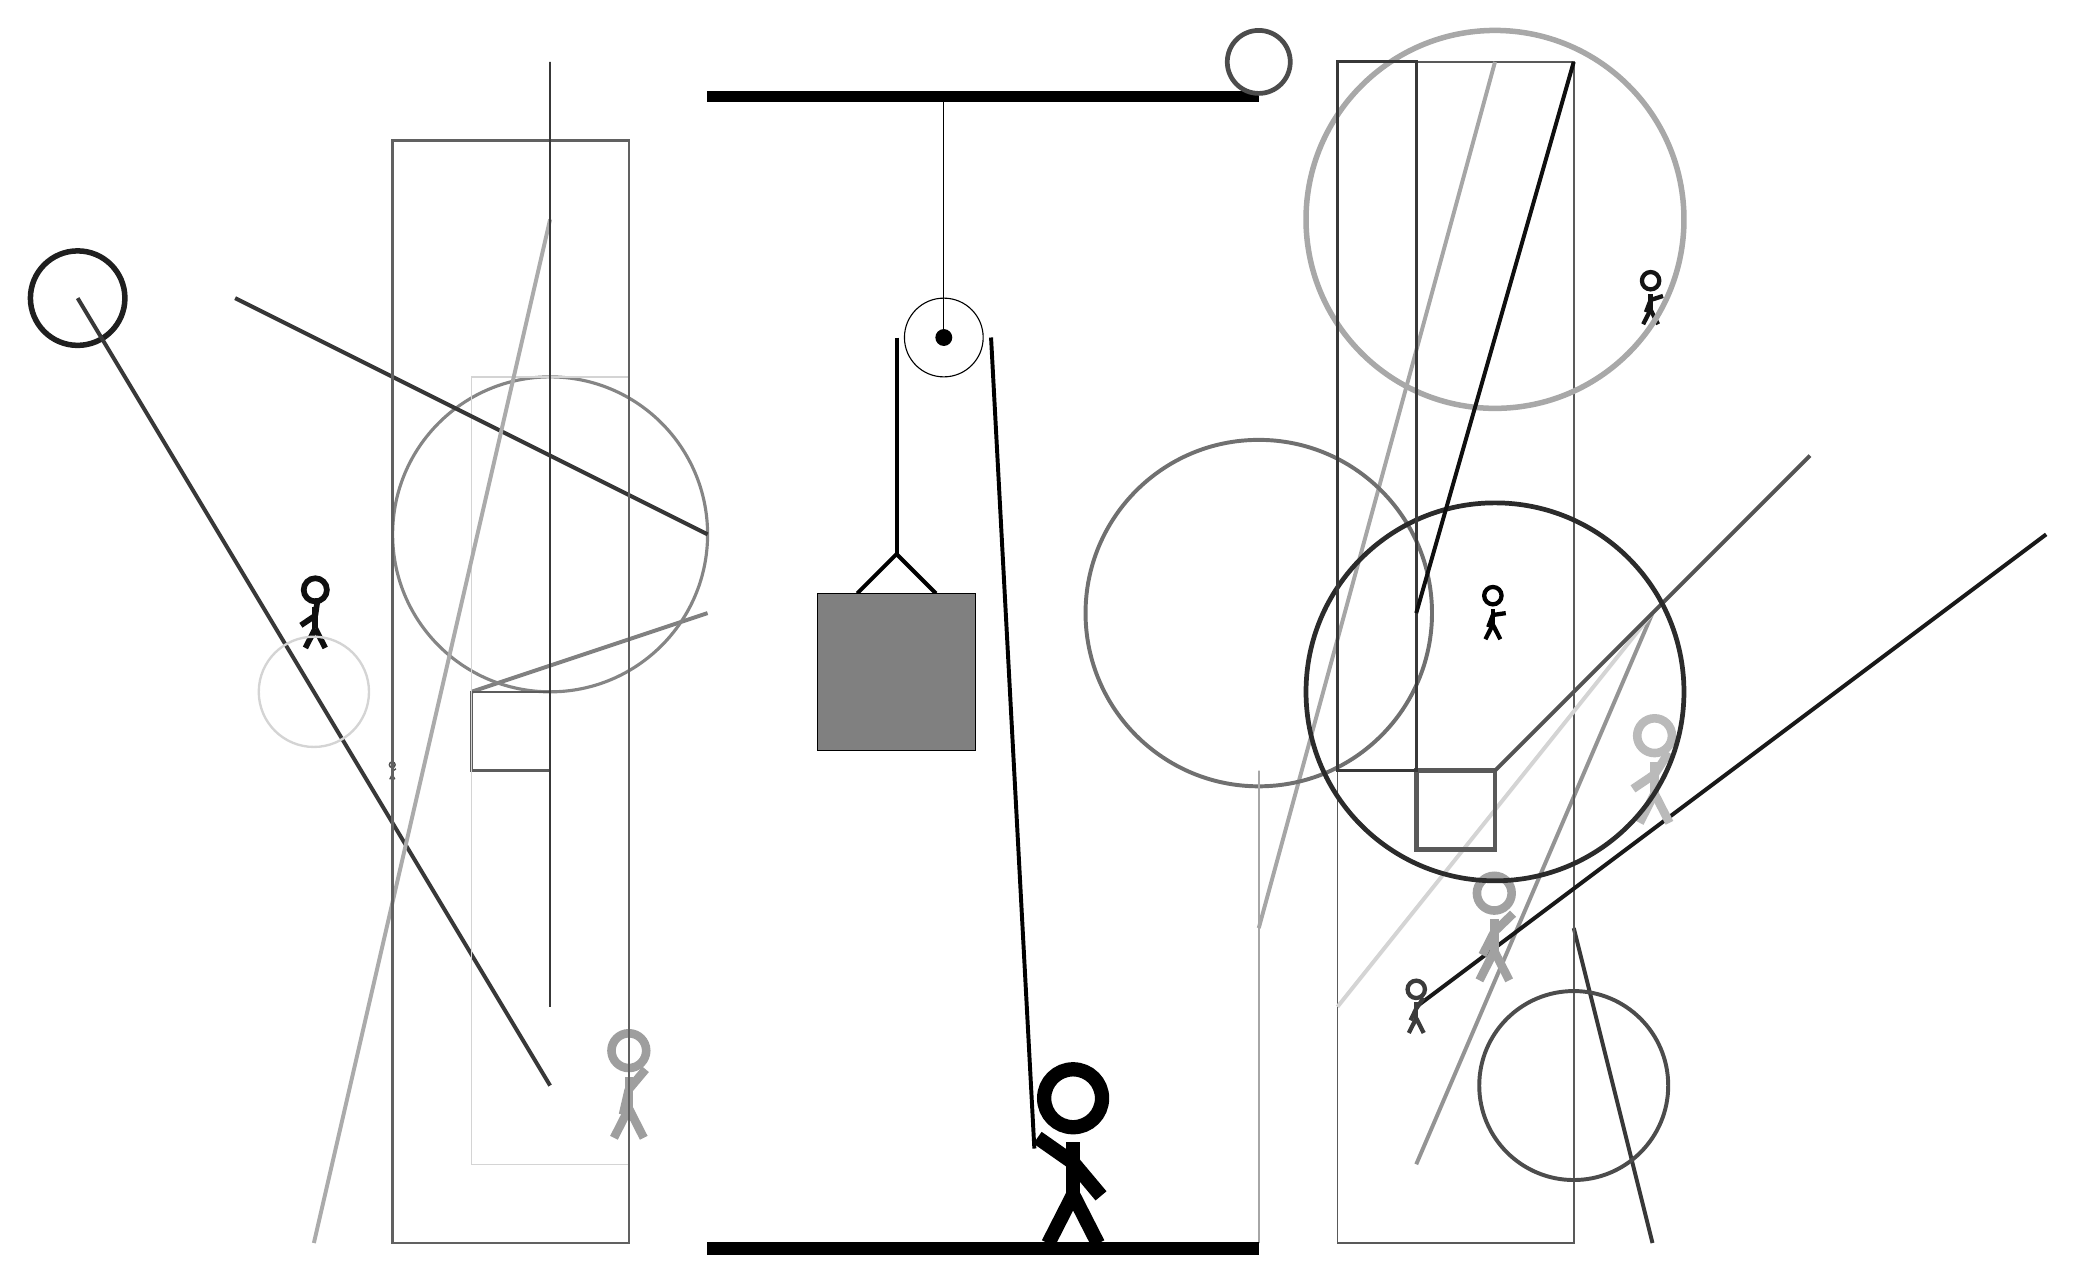
\begin{tikzpicture}
			%%%%% START %%%%%
			
			\draw[fill=black] (-2, 11.5) rectangle (5, 11.625);
			
			\draw (1, 8.5) circle (0.5);
			\draw[fill=black] (1, 8.5) circle (0.1);
			\draw (1, 11.5) -- (1, 8.5);
			
			\draw[line width=0.5mm] (-0.1, 5.25) -- (0.4, 5.75) -- (0.9, 5.25);
			\draw[fill=black!50] (-0.6, 5.25) rectangle (1.4, 3.25);
			
			\draw[line width=0.5mm] (0.4, 8.5) -- (0.4, 5.75);
			\centerarc[line width=0.5mm](1, 8.5)(0:180:0.6);
			\draw[line width=0.5mm](1.6, 8.5) -- (2.15, -1.8);
			
			\node at (2.6, -1.9) {\Strichmaxerl[10][-35][-50]};
			
			\draw [line width=0.7mm, color=black!88](-10, 9) circle (0.6);
			
			\draw[line width=0.5mm, color=black!50](-2, 5) -- (-5, 4);
			\draw[line width=0.5mm, color=black!78](9, 1) -- (10, -3);
			\draw[line width=0.5mm, color=black!42](10, 5) -- (7, -2);
			\node[line width=0.6mm, color=black!92] at (10, 9) {\Strichmaxerl[3][69][18]};
			\draw [line width=0.4mm, color=black!48](-4, 6) circle (2.0);
			\draw[line width=0.3mm, color=black!64] (-4, 4) rectangle (-5, 3);
			
			\draw[line width=0.5mm, color=black!78](-4, -1) -- (-10, 9);
			\node[line width=0.7mm, color=black!38] at (-3, -1) {\Strichmaxerl[6][77][50]};
			\draw[line width=0.2mm, color=black!65] (6, 12) rectangle (9, -3);
			
			\draw[line width=0.5mm, color=black!90](7, 0) -- (15, 6);
			
			\draw[line width=0.5mm, color=black!17](6, 0) -- (10, 5);
			\draw[line width=0.2mm, color=black!17] (-3, 8) rectangle (-5, -2);
			
			\node[line width=0.5mm, color=black!100] at (8, 5) {\Strichmaxerl[3][69][8]};
			\draw[line width=0.6mm, color=black!65] (7, 2) rectangle (8, 3);
			\node[line width=0.5mm, color=black!94] at (-7, 5) {\Strichmaxerl[4][34][82]};
			
			\node[line width=0.6mm, color=black!69] at (-6, 3) {\Strichmaxerl[1][87][33]};
			
			\node[line width=0.2mm, color=black!37] at (8, 1) {\Strichmaxerl[6][63][44]};
			\draw[line width=0.5mm, color=black!79](-2, 6) -- (-8, 9);
			\draw[line width=0.5mm, color=black!35](8, 12) -- (5, 1);
			\draw[line width=0.5mm, color=black!67](8, 3) -- (12, 7);
			
			\draw [line width=0.7mm, color=black!34](8, 10) circle (2.4);
			\draw[line width=0.5mm, color=black!33](-7, -3) -- (-4, 10);
			\node[line width=0.2mm, color=black!27] at (10, 3) {\Strichmaxerl[6][34][57]};
			\draw[line width=0.3mm, color=black!62] (-3, 11) rectangle (-6, -3);
			\draw [line width=0.5mm, color=black!70](9, -1) circle (1.2);
			\draw [line width=0.3mm, color=black!17](-7, 4) circle (0.7);
			\draw [line width=0.5mm, color=black!56](5, 5) circle (2.2);
			
			\node[line width=0.7mm, color=black!77] at (7, 0) {\Strichmaxerl[3][64][56]};
			
			\draw[line width=0.2mm, color=black!78] (-4, 12) rectangle (-4, 0);
			\draw [line width=0.6mm, color=black!83](8, 4) circle (2.4);
			
			\draw [line width=0.6mm, color=black!70](5, 12) circle (0.4);
			\draw[line width=0.4mm, color=black!78] (7, 12) rectangle (6, 3);
			\draw[line width=0.3mm, color=black!35] (5, 3) rectangle (5, -3);
			\draw[line width=0.5mm, color=black!94](9, 12) -- (7, 5);
			
			\draw[fill=black] (-2, -3) rectangle (5, -3.15);
			
			%%%%% END %%%%%
		\end{tikzpicture}
	\end{figure}	
\end{document}